
\begin{figure}
\centering
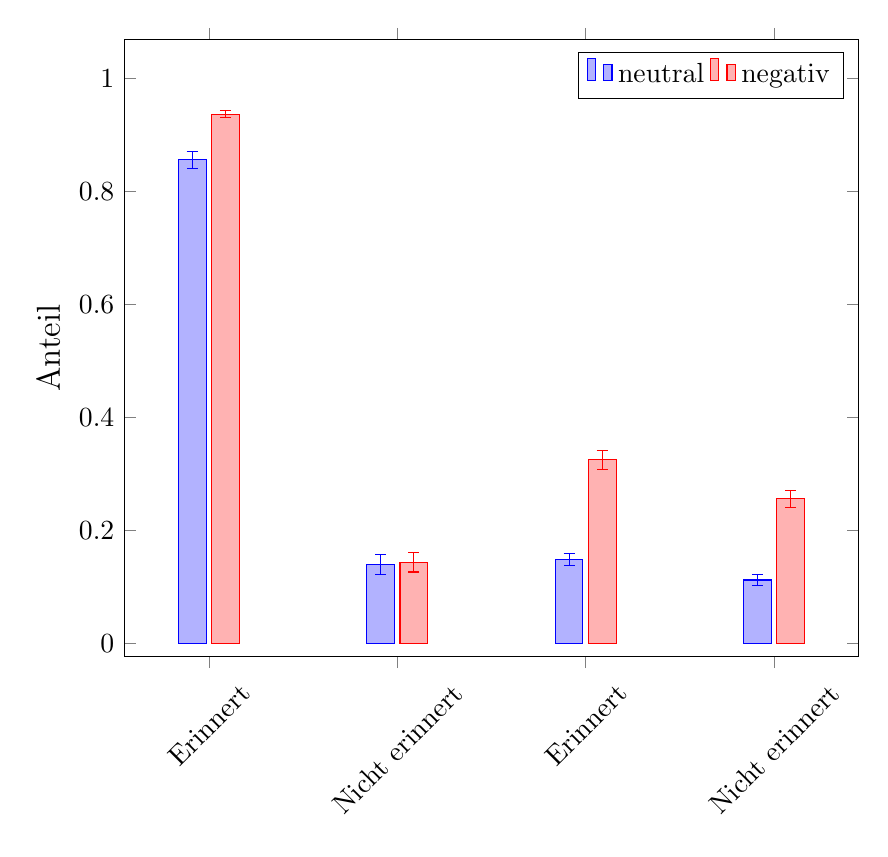
\begin{tikzpicture}
\begin{axis}[
    % instead of scaling
    width=0.9\linewidth,
    ybar,
    enlargelimits=0.15,
    legend style={
    % to save space I would place the legend inside the axis, at least with these data
      %at={(0.5,-0.2)},
      %anchor=north,
      legend columns=-1
    },
    ylabel={Anteil},
    ylabel style={font=\large},
    xtick=data,
    % use explicit ticklabels instead of symbolc x coords
    xticklabels={Erinnert,Nicht erinnert,Erinnert,Nicht erinnert},
    xticklabel style={
    %  text width=2cm,
      % yshift=-18pt, % move sticks down a bit
    %  align=center
    rotate=45
    },
    %%%%%%% extra ticks
    % extra x ticks={1.5,3.5},
    % extra x tick labels={Freie Wiedergabe Tag 1,Freie Wiedergabe Tag 2},
    % extra x tick style={
    %   %%%%%%%% because the xticklabel style also affects the extra ticks, 
    %   %%%%%%%% shift extra ticklabels back up
    %   ticklabel style={yshift=13pt},
    %   %%%%%%%% tickwidth is actually the length of of the ticks (the small lines)
    %   tickwidth=0
    % }
]
%neutral
\addplot[blue,fill=blue!30!white,error bars/.cd,y dir=both,y explicit,]
coordinates{
   (1,0.8560) +-(0.01503,0.01503)
   (2,0.1390) +-(0.01737,0.01737)
   (3,0.1481) +-(0.01067,0.01067)
   (4,0.1119) +-(0.00922,0.00922)
};
%negativ
\addplot[red,fill=red!30!white,error bars/.cd,y dir=both,y explicit,]
coordinates {
  (1,0.9365) +- (0.00587,0.00587)
  (2,0.1435) +- (0.01737,0.01737)
  (3,0.3247) +-(0.01695,0.01695)
  (4,0.2556) +-(0.01524,0.01524)
};
\legend{neutral,negativ}
\end{axis}
\end{tikzpicture}
\caption{Unterschrift A}
\label{GedaechtnisBilder}
\end{figure}